%\settikzpagecorners

In this section, we discuss how to fit various types of curves to data.

\section{Matlab: Curve Fitting}\label{sec:Matlab_curvefitting}

The main commands for this section are \cour{polyfit}, \cour{polyval} and \cour{interp1}.
Let's begin with linear regression.\\

\index{Matlab Functions!\cour{polyfit}}
\example{ex_linearregression}{\textbf{Linear Regression}\\

Plot a set of data:\\
\\
\cour{>> x=0:5;y=[12,10,9,6,2,0];}\\
\cour{>> plot(x,y,{\color{myred} \tq o\tq})}\\
\\
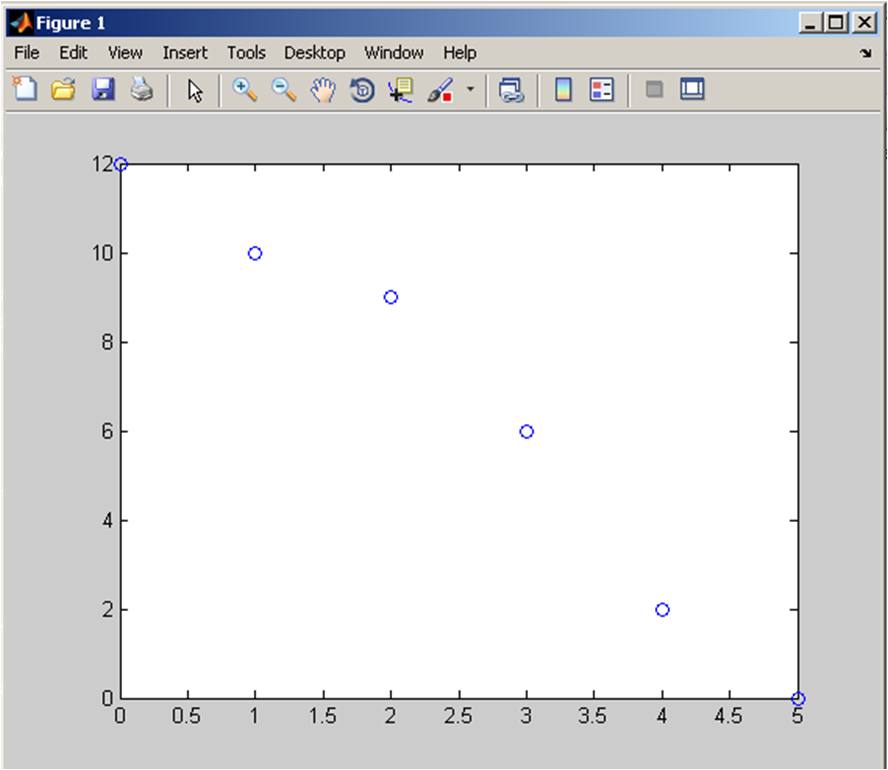
\includegraphics[scale=.5]{figures/matlab_linreg1}

The data certainly seems to have a (downward) linear trend.  We can find the line of best fit as follows: \\
\cour{>>coeffs=polyfit(x,y,1);}\\
\cour{>>besty=coeffs(1)*x+coeffs(2);}\\

The command \cour{polyfit} returns the matrix \cour{[-2.4857 12.7143]} of the slope and $y$-intercept of the line of best fit.  The $y$ values of this line corresponding to $x$ (from 0 to 5) are stored in the variable \cour{besty}.  We plot them together using:\\
\\
\cour{>>plot(x,y,{\color{myred} \tq o\tq},x,besty)}\\
\\
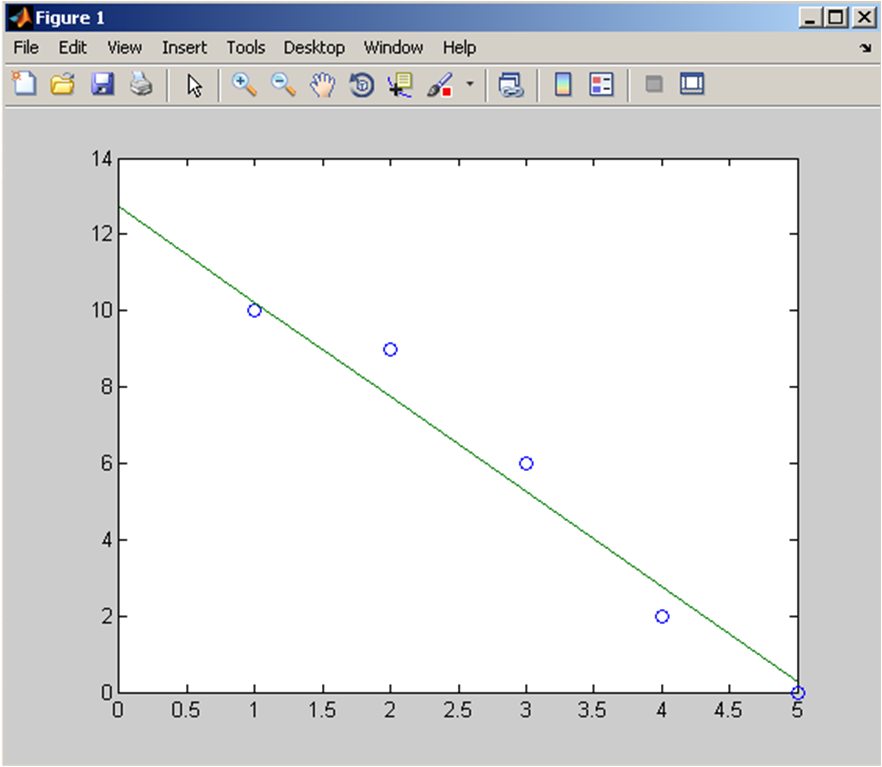
\includegraphics[scale=.5]{figures/matlab_linreg2}
}\\

We often use regression lines to guess $y$ values for $x$ values that are not included in the data set.  For this, we use interpolation.\\

\index{Matlab Functions!\cour{interp1}}
\example{ex_interp1}{\textbf{Interpolation}\\

Using the data from example \ref{ex_linearregression}, we would like to know the $y$ value corresponding to the $x$ value 3.5.  For this, we use the command \cour{interp1} (that's the number one on the end, not a lowercase for the letter L).\\
\\
\cour{>> interp1(x,y,3.5,{\color{myred} \tq linear\tq})}\\
\cour{ans =}\\
\cour{\ps 4}\\

We plot these together with the interpolated point indicated with a red triangle.\\
\\
\cour{plot(x,y,{\color{myred} \tq o\tq},x,besty,3.5,4,{\color{myred} \tq r>\tq})}\\
\\
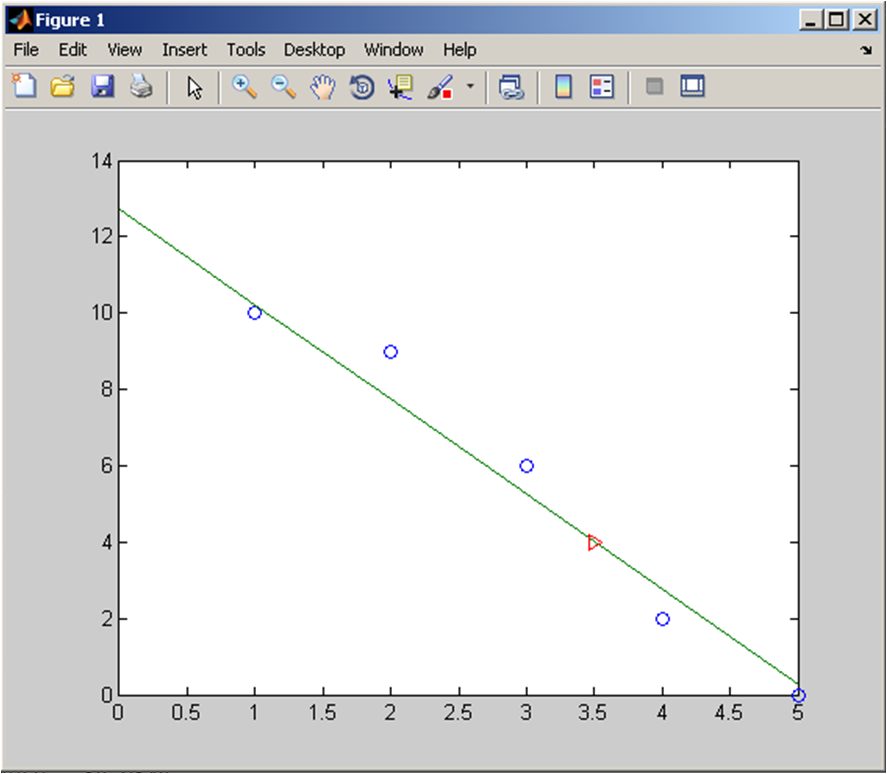
\includegraphics[scale=.5]{figures/matlab_linreg3}
}\\

Note that if you try to use the \cour{interp1} function for data that is outside the data set, you will get an error since you are trying to ``extrapolate'' instead of interpolate.\\
\\
\cour{>>interp1(x,y,10.5,{\color{myred} \tq linear\tq})}\\
\\
gives\\
\\
\cour{ans =}\\
\cour{\ps NaN}\\

This indicates that the answer is \cour{NaN} or ``Not a Number'' (look it up in the Help files).\\
\\
\noindent \large \textsf{\textbf{Higher Order Polynomial Fitting}} \normalsize\\

Let's try fitting a fifth degree polynomial to the data in example \ref{ex_linearregression}.\\

\example{ex_fifthorder}{\po\\
\\
\cour{>> x=0:5;y=[12,10,9,6,2,0];}\\
\cour{>> coeffs5=polyfit(x,y,5)}\\
\\
returns\\
\\
\cour{coeffs5 =}\\
\cour{\ps    -0.0167    0.3333   -2.0833    4.6667   -4.9000   12.0000}\\
\\
which are the coefficients for the approximating 5th order polynomial, namely 
$y = -0.0167 x^5 + 0.3333 x^4 - 2.0833 x^3 + 4.6667 x^2 - 4.9 x +  12$.\\
\\

\index{Matlab Functions!\cour{polyval}}
We could type out the full polynomial, but there is a shortcut.  We can use the function \cour{polyval} along with \cour{linspace} to give a smooth approximating curve.\\
\\
\cour{>> x5=linspace(0,5);}\\
\cour{>> y5=polyval(coeffs5,x5);}\\

We plot the curves\\
\cour{>> plot(x,y,'o',x,besty,x5,y5)}\\
\\
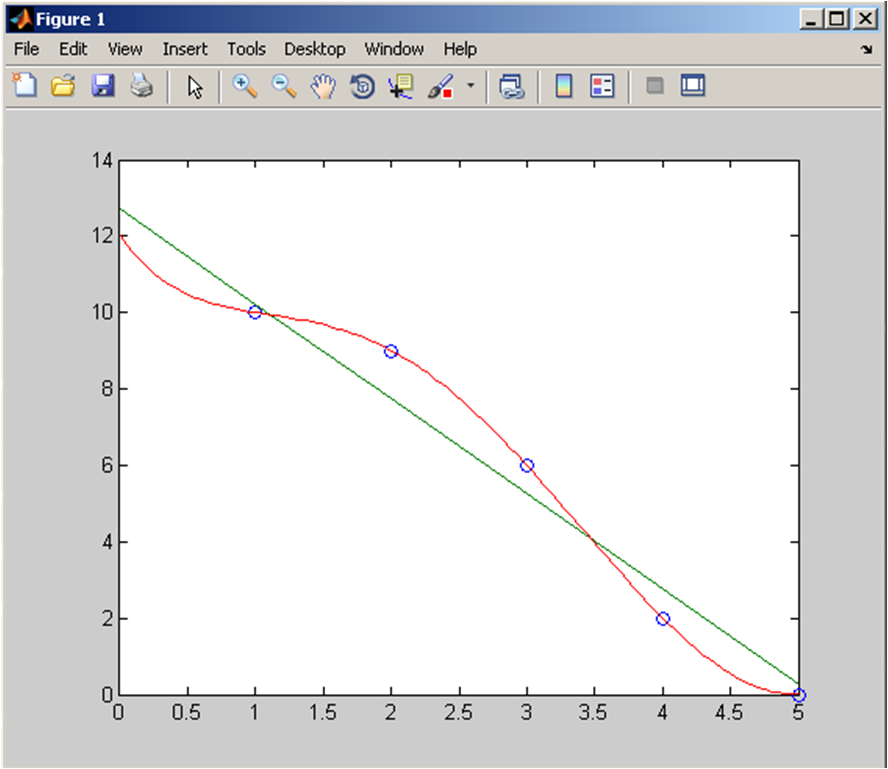
\includegraphics[scale=.5]{figures/matlab_polyreg}
}\\

\noindent \large \textsf{\textbf{Interactive Fitting Tools}} \normalsize\\

If you aren't sure about the fit you want, you can use the interactive fitting tools.
We start again by closing any figure windows, clearing out the variables and clearing the Command Window.  A short cut to do this could be:\\
\\
\cour{>> close {\color{myred} all},clear,clc}\\

Re-enter the data.\\
\\
\cour{>> x=0:5;}\\
\cour{>> y=[12,10,9,6,2,0];}\\
\cour{>> plot(x,y,{\color{myred} \tq o\tq})}\\

On the figure screen, go to the menu item Tools $>$ Basic Fitting.  This will launch a new window:\\
\\
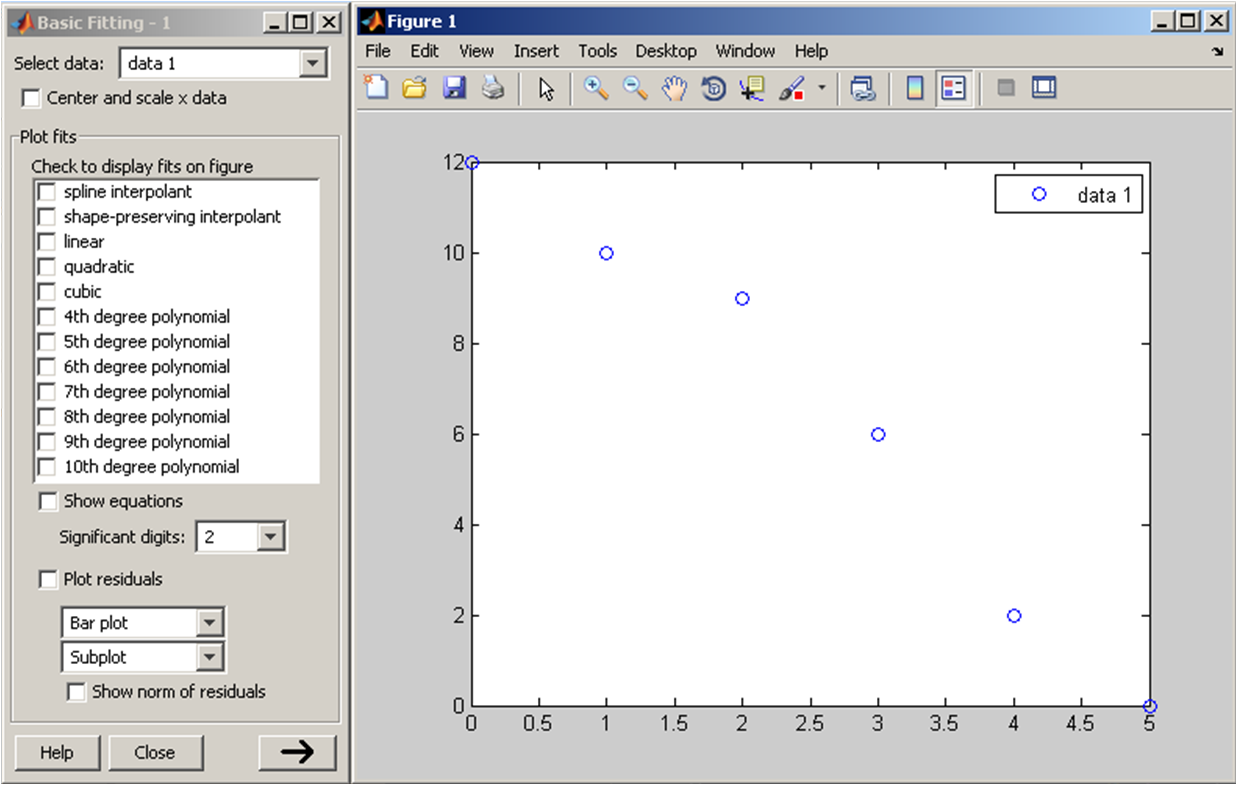
\includegraphics[scale=.5]{figures/matlab_interactivefit}\\

Now you simply have to select the polynomial(s) that you want to fit (try a few!).  You can even see the corresponding equations (and more) using the big arrow button 
\includegraphics[scale=.6]{figures/matlab_arrowbutton}.  If we select the ``linear'' and ``5th degree polynomial'' check boxes, and the ``Show equations'' check box, we will see the equations on the graph itself.\\

\hspace{-.2in}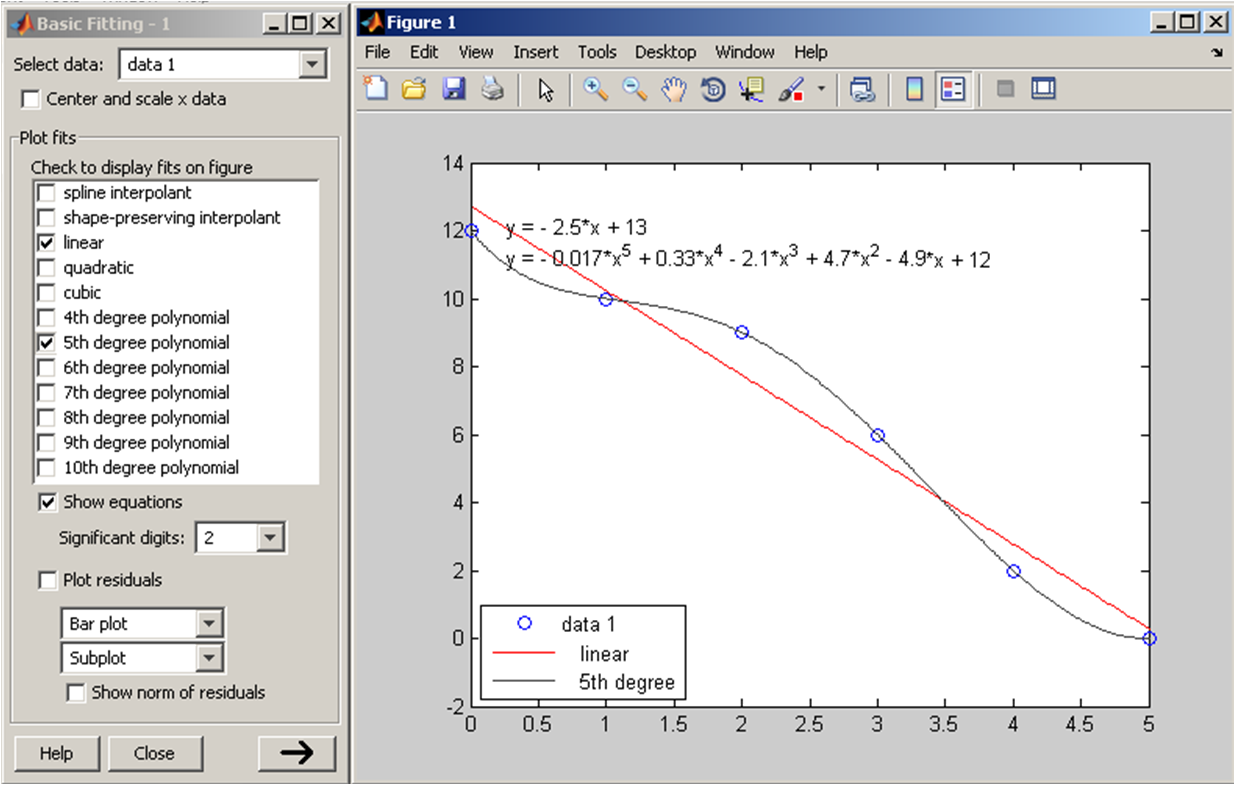
\includegraphics[scale=.5]{figures/matlab_polyreg2}

\newpage
\printexercises{exercises/09_exercises}
%\example{a}{b}{c}

%\definition{def:lineintegral}{\textbf{TITLE}}
%
%\keyidea{idea:lineintprops}{\textbf{TITLE}}
%
%\printexercises{exercises/mathcad_introduction_exercises}
